\section{Results}
In this section I will present the results from running the various classification models on the Wikipedia dataset and then proceed to investigate how well these models perform on a dataset from a different domain.

\subsection{Baseline With langid.py}

As a baseline to compare the performance of the models in this word I would like to compare with an out of the box language classification system. "langid.py: An Off-the-shelf Language Identification Tool." \cite{langID} is such a tool.\\

Out of the box langid.py comes with with a pretrained model which covers 97 languages. The data for langid.py comes from from 5 different domains: government documents, software documentation, newswire, online encyclopedia and an internet crawl.\\

I have written a program to test how well langid.py performed on the Wikipedia dataset using the the python API.\footnote{\url{https://pypi.org/project/langid/}}\\

Since langid.py returned the language id "no" (Norwegian) on some of the data points i chose to restrict langid.py to only be able to return either "nn" (Nynorsk) or "nb" (Bokmål) as predictions. It is a quite peculiar feature of the Norwegian language that there exist two different written languages but three different language codes.

\begin{figure}[h!]
  \centering
  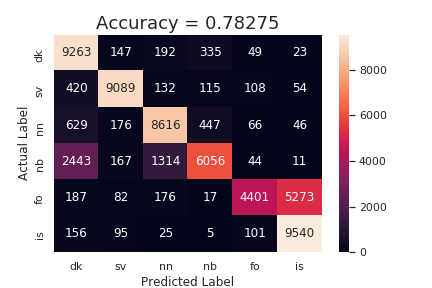
\includegraphics[width = 200pt]{figs/langid}
  \caption{Confusion matrix with results from langid.py on the full dataset with 300K data points. }
  \label{langid_confusion_matrix}
\end{figure}

In Figure \ref{langid_confusion_matrix} we see the confusion matrix for the langid.py classifier. The largest errors are between Danish and Bokmål and between Faroese and Icelandic. We see that langid.py was actually able to correctly classify most of the Danish data points however approximately a quarter of the data points in Bokmål was incorrectly classified as Danish and just under and eighth was classified as Nynorsk.\\

Furthermore langid.py correctly classified most of the Icelandic data points however over half of the data points in Faroese was incorrectly classified as Icelandic.

\subsection{Baseline with linear models.}

In the Figure \ref{baseline-results-10k} we see the results for running the models on a dataset with 10K data points in each language category. We see that the models in general perform better if we use character level bi-grams instead of uni-grams (individual) characters.\\

Also we see that logistic regression and support vector machines outperform Naive Bayes and K nearest neighbors in all cases. Furthermore for all models we get the best performance if we use the skipgram model from FastText.\\

If we compare the cbow mode from FastText with character level bi-grams we see that the cbow model is on par with bi-grams for the KNN and Naive Bayes classifiers while bi-grams outperform the cbow for Logistic Regression and support vector machines.\\

\begin{figure}[h!]
  \centering
  \begin{tabular}{ l | c | r }
    \hline
    Model               & Encoding  & Accuracy \\
    \hline
    Knn                 & cbow &  0.780\\
    Log-Reg             & cbow &  0.819\\
    Naive Bayes         & cbow &  0.660\\
    SVM                 & cbow &  0.843\\
    Knn                 & skipgram &  0.918\\
    Log-Reg             & skipgram &  \textbf{0.929}\\
    Naive Bayes         & skipgram &  0.840\\
    SVM                 & skipgram &  \textbf{0.928}\\
    Knn                 & char bi-gram  & 0.745\\
    Log-Reg             & char bi-gram  & 0.907\\
    Naive Bayes         & char bi-gram  & 0.653\\
    SVM                 & char bi-gram  & 0.905\\
    Knn                 & char uni-gram  & 0.620\\
    Log-Reg             & char uni-gram  & 0.755\\
    Naive Bayes         & char uni-gram  & 0.614\\
    SVM                 & char uni-gram  & 0.707\\
    \hline
  \end{tabular}
  \caption{Overview of results for the dataset with 10K data points in each language.}
  \label{baseline-results-10k}
\end{figure}

\subsection{Results with neural networks.}
In the following we evaluate the initial results for the neural network architectures which can be seen in Figure \ref{keras-results}. Here we compare the result of doing character level uni- and bi-grams using the Multilayer Perceptron and Convolutional Neural Network. We see that the CNN performs the best, achieving an accuracy of 95.6\% when using character bi-grams. Both models perform better using bi-grams than individual characters as features while the relative increase in performance is greater for the MLP model.

\begin{figure}[h!]
  \centering
  \begin{tabular}{ l | c | r }
    \hline
    Model               & Encoding  & Accuracy \\
    \hline
    MLP                 & char bi-gram &  0.898 \\
    CNN                 & char bi-gram & \textbf{0.956} \\
    % LSTM                & char bi-gram & 60k & 0.933 \\
    MLP                 & char uni-gram &  0.697\\
    CNN                 & char uni-gram  & 0.942 \\
    % LSTM                & char uni-gram & 60k &  \\
    \hline
  \end{tabular}
  \caption{Overview of results for the neural network models for the dataset with 10K data points in each language.}
  \label{keras-results}
\end{figure}


\subsection{Increasing the size of the dataset.}
Usually the performance of supervised classification models increase with more training data. In this section I have increased amount of training data to 50K sentences in each of the language categories. Due to much longer training times I choose to only rerun the "baseline models" with the skipgram encoding from FastTest which we saw achieved the highest accuracy.

\begin{figure}[h!]
  \centering
  \begin{tabular}{ l  c | r }
    \hline
    Model               & Encoding & Accuracy \\
    \hline
    Knn                 & skipgram & 0.931\\
    Logistic Regression & skipgram  & \textbf{0.933}\\
    Naive Bayes         & skipgram  & 0.806\\
    SVM                 & skipgram& 0.925\\
    \hline
  \end{tabular}
  \caption{Overview of results for the dataset with 50K data points in each language.}
  \label{results-sklearn300k}
\end{figure}

As can be seen in Figure \ref{results-sklearn300k} the accuracies for the logistic regression model and the K nearest neighbors algorithm improved by including more data, however not by much. Unexpectedly the accuracies for the support vector machine and naive Bayes actually dropped a bit by including more data.\\

Even when including five times the amount of data the best result, logistic regression with an accuracy of 93.3\%, is still worse than for the Convolutional Neural Network trained on 10K data points in each language.\\

In Figure \ref{results-keras-300k} we see the results for running the neural networks on the larger dataset. Both models improve by increasing the amount of data and the Convolutional Neural Network reached an accuracy of 97\% which is the best so far.

\begin{figure}[h!]
  \centering
  \begin{tabular}{ l c | r }
    \hline
    Model               & Encoding & Accuracy \\
    \hline
    MLP                 & char bi-gram  & 0.918\\
    CNN                 & char bi-gram  & \textbf{0.970}\\
    \hline
  \end{tabular}
  \caption{Overview of results for the dataset with 50K data points in each language.}
  \label{results-keras-300k}
\end{figure}

% In Figure \ref{training} we see a plot of the accuracy during training on the training and validation set respectively. We see that the accuracy on the validation set follows the accuracy on the training set more closely for the CNN than for the MLP.

% \begin{figure}[h!]
%     \centering
%     \begin{subfigure}[b]{100pt}
%         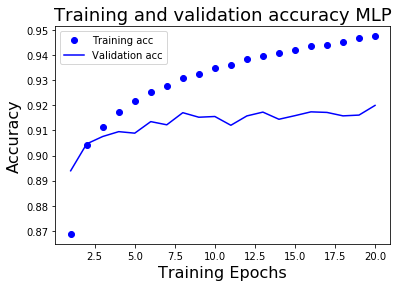
\includegraphics[width=\textwidth]{figs/training_MLP}
%         \caption{Training accuracy MLP}
%     \end{subfigure}
%     ~
%     \begin{subfigure}[b]{100pt}
%         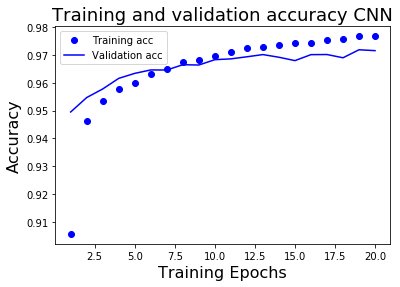
\includegraphics[width=\textwidth]{figs/training_CNN}
%         \caption{Training accuracy CNN}
%     \end{subfigure}
%     \caption{Accuracy on test and validation set during training of the different neural networks on the full dataset with 50K data points in each language.}
%     \label{training}
% \end{figure}

In Figure \ref{confusion_matrix-big-cnn} we see the confusion matrix for the convolutional Neural Network trained on the full Wikipedia dataset with 300K data points pr language. We see that the largest classification errors still happens between Danish, Bokmål and Nynork as well as between Icelandic and Faroese. \\

\begin{figure}[h!]
  \centering
  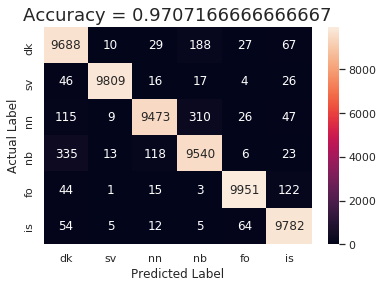
\includegraphics[width = 200pt]{figs/confusion_CNN}
  \caption{Confusion matrix with results from the convolutional neural network on the full datasetwith 50K data points in each language.}
  \label{confusion_matrix-big-cnn}
\end{figure}

\subsection{Optimizing the kernel size.}
In attempt to optimize the CNN i tried to look at different kernel sizes (between 1 and 11) for character level uni- bi- and trigrams. I tested on the dataset with 10K sentences in each language since the training time for a single CNN was several hours and it would have taken several days to train on the full dataset even using cloud resources in Google Colab. We see the results in Figure \ref{kernel_sizes}.\\

\begin{figure}[h!]
  \centering
  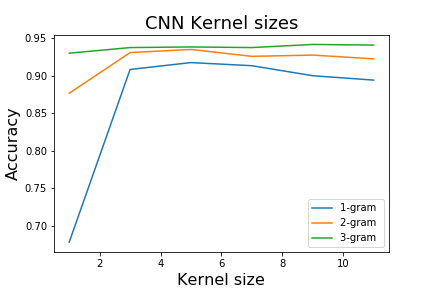
\includegraphics[width = 225pt]{figs/KernelSizes}
  \caption{Accuracy for different kernel sizes for the Constitutional Neural Network.}
  \label{kernel_sizes}
\end{figure}

\subsection{Using FastText supervised}

FastText can also be used for be trained supervised and be used for Classification. In the Paper Bag of Tricks for Efficient Text Classification \cite{BagOfTricks} the authors show that FastText can obtain performance on par with methods inspired by deep learning, while being much faster on a selection of different tasks in Tag prediction and Sentiment Analysis. The confusion matrix from running the FastText supervised classifier can be seen in Figure \ref{fasttext_supervised}. We see that FastText is on par with the CNN\\


\begin{figure}[h!]
  \centering
  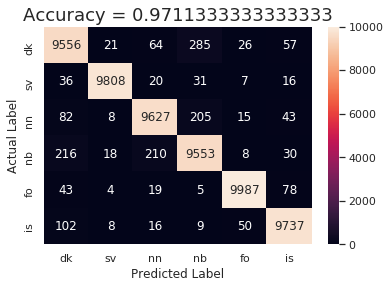
\includegraphics[width = 225pt]{figs/fasttext_supervised}
  \caption{Confusion matrix with results from a supervised FastText model on the full dataset with 300K datapoints.}
  \label{fasttext_supervised}
\end{figure}

\subsection{Reflections.}
At this point I it beneficial to take a step back and look at what we have done so far. We have developed a selection of different models and our results to far indicate that the FastText supervised model and the CNN both give quite good results on the Wikipedia dataset with accuracies over 97\%. \\

In the rest of this section I would like to investigate the cases there these classifiers fail and try if I can find common patters. Also i will test the models on a dataset which they have not been trained on to investigate how well the models generalize to data from a different domain than Wikipedia. \\


\subsection{Looking at failure cases}
Now having achieved quite good results with FastText and the CNN I now look a bit more closely at the sentences which were misclassified by both models. \\

As a first observation the misclassified sentences tend to be shorter than the correctly classified ones. In Figure \ref{faliurelengthdist} I have plotted the distribution of the length, defined as the number of characters after the data cleaning procedure as defined in a previous section. The mean length of the sentences in the test set is 104.74 characters with a standard deviation of 65.39 while it is only 48.91 characters with a deviation  of 37.27. \\

\begin{figure}[h!]
    \centering
    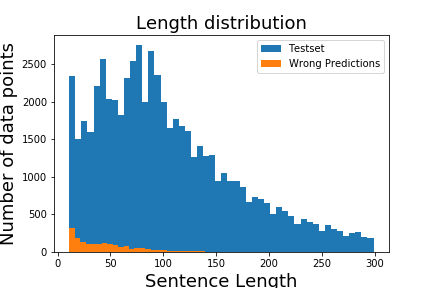
\includegraphics[width=200pt]{figs/faliurelengthdist}
    \caption{Distribution of sentence lengths.}
    \label{faliurelengthdist}
\end{figure}

Generally the misclassified sentences fall into the categories: Very short sentences, names, mathematical content and sentences with many foreign words.\\

\textbf{Mathematical equations}:
A substantial (and useful) part of Wikipedia is related to mathematics and equations are common on these pages. My Wikipedia scraper did not filter out mathematical equations which appear in the dataset as in the examples below. \\

\begin{verbatim}
displaystyle n lambda eff cdot t
displaystyle a frac a cot frac pi simeq a
displaystyle a b c a cdot b a cdot c ab ac
\end{verbatim}

\textbf{Foreign Words}:
Another common type of misclassified sentences with a lot of foreign words. In the dataset this commonly happened with English words. Below are some examples of misclassified sentences where most or all word are from foreign languages. \\

\begin{verbatim}
art garfunkel all i know skywriter
 watermark

mémoires de la société des antiquaires
du nord fjögur bindi

avatar the last airbender prins zuko

the fifth dimension up up and away
\end{verbatim}
% heimsnet e mbwa mobile broadband wireless access
% y is yhat dk
%  y is yhat nb
% y dk yhat fo
%  y nb yhat fo


\textbf{Names}: Another common failure case is sentences that contain only names of people or locations. Examples are
\begin{verbatim}
  romain rolland
  henry morton stanley
  anna karin
\end{verbatim}
% y is yhat fo
% y sv yhat fo
% y is yhat fo

It is not surprising that these cases are hard to classify since names are usually spelled the same way irrespective of language. \\

\textbf{Danish and Bokmål}:
One of the largest error categories was sentences on Danish or Bokmål misclassified as the other language.\\

This is not surprising sine these two languages are very closely related and often the difference between them is an alternative spelling of a single word in a sentence. \\

The examples below are in Bokmål but was classified as Danish. The first sentence is in indistinguishable from danish except from the alternative spelling of the single word  "magesekken" which would be "mavesækken" in Danish. \\

The Second sentence would be hard or impossible for a native speaker to distinguish since the there is no difference between this sentence in the two languages.Finally for the third example the difference is only two characters in the word "sommerfuglhager" which in danish would be spelled as "sommerfuglehaver".

\begin{verbatim}
(1) hos mennesket har magesekken et
    volumet ca

(2) klubben har hjemmebane på slettebakken
    hvor de også har et klubbhus

(3) en dyrepark kan derfor også omfatte
    for eksempel akvarier terrarier
    sommerfuglhager og fuglehus
\end{verbatim}

\subsection{Evaluating the models on another dataset}
It would be interesting to see how the two best performing models generalize by testing on a dataset different from the they have been trained on (the Wikipedia dataset).\\

I downloaded an additional dataset from Tatoeba\footnote{{\tt tatoeba.org/}} which is a large database of user provided sentences and translations. In Figure \ref{tatoebasentprlang} we see the number of sentences in each language for all sentences in the Tatoeba dataset. Observe that we have very few samples in Nynorsk and Faroese.\\

\begin{figure}[h!]
    \centering
    \begin{subfigure}[b]{0.45\textwidth}
      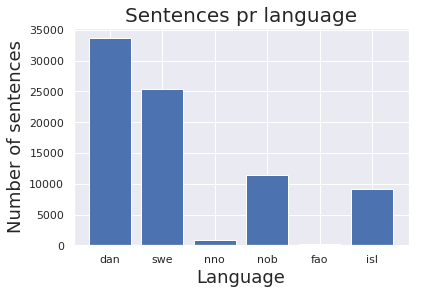
\includegraphics[width =\textwidth]{figs/tatoebasentprlang}
      \caption{Distribution of the number of sentences in each language in the tatoeba dataset.}
      \label{tatoebasentprlang}
    \end{subfigure}
    ~
    \begin{subfigure}[b]{0.45\textwidth}
      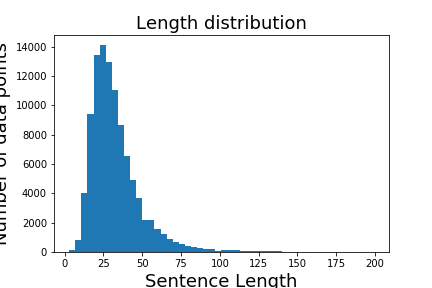
\includegraphics[width =\textwidth]{figs/taboeba-faliurelengthdist}
      \caption{Distribution of the length of  sentences tatoeba dataset.}
      \label{tatoebalengths}
    \end{subfigure}
        \caption{Distribution of the lengths and language classes of Tatoeba sentences.}
\end{figure}

The language used in the Tatoeba dataset is different from the language used in Wikipedia. The Tatoeba dataset mainly consists of sentences written in everyday language. Below we see some examples from the Danish part of the Tatoeba dataset.
\begin{verbatim}
Hvordan har du det?

På trods af al sin rigdom
og berømmelse, er han ulykkelig.

Vi fløj over Atlanterhavet.

Jeg kan ikke lide æg.

Folk som ikke synes at latin er det
smukkeste sprog, har intet forstået.
\end{verbatim}

The confusion matrix for the FastText supervised model and the CNN, which are both trained on the full Wikipedia dataset and then evaluated on the Tatoeba dataset can be seen in Figure \ref{tatoeba-confuss}. Both models use the same setting that produced good results on the Wikipedia dataset.

\begin{figure}[h!]
    \centering
    \begin{subfigure}[b]{0.45\textwidth}
        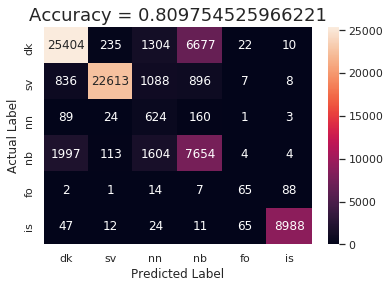
\includegraphics[width=\textwidth]{figs/tatoeba-langid}
        \caption{Langid.py}
    \end{subfigure}
    ~
    \begin{subfigure}[b]{0.45\textwidth}
        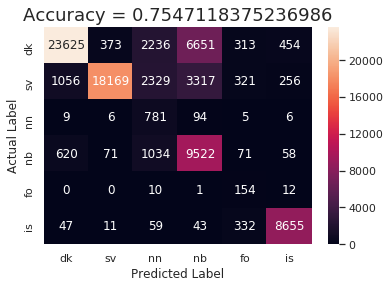
\includegraphics[width=\textwidth]{figs/tatoeba-fasttext}
        \caption{fasttext classifier }
    \end{subfigure}
    ~
    \begin{subfigure}[b]{0.45\textwidth}
        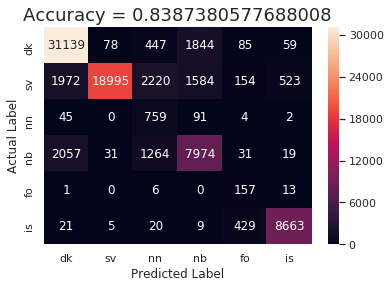
\includegraphics[width=\textwidth]{figs/tatoeba-cnn}
        \caption{Convolutional neural network}
    \end{subfigure}
    \caption{Confusion matrices for the tatoeba dataset }
    \label{tatoeba-confuss}
\end{figure}

We see that the performance drops quite a lot when shifting to another domain. For reference the accuracy of langid.py on this dataset is 80.9\% so FastText actually performs worse than the baseline with an accuracy of 75.5\% while the CNN is a bit better than the baseline with an accuracy of 83.8 \% \\

One explanation for the drop in performance is that the sentences in the Tatoeba dataset is significantly shorter than the sentences in the Wikipedia dataset as seen in Figure \ref{tatoebalengths}. As we saw in the previous section both models tend to misclassify shorter sentences more often than longer sentences. This and the fact that the "genre" of sentences are different might explain why the models trained on the Wikipedia dataset does not generalize too well to the Tatoeba dataset without a drop on performance.\\

The CNN uses character bi-grams as features while, with the standard settings, FastText uses only individual words to train. The better performance of the CNN might indicate that character level n-grams are more useful features for language identification than words alone.\\

To test this I changed the setting of FastText to train using only character level n-grams in the range 1-5 instead of individual words. In Figure \ref{fasttextcharngram} we see the confusion matrix for this version of the FastText model. This version still achieved 97.8\% on the Wikipedia test set while improving the accuracy on the Tatoeba dataset from 75.4\% to 85.8\% which is a substantial increase.\\

Thus using character level features seem to improve the FastText models ability to generalize to sentences belonging to a domain different from the one it has been trained on.

\begin{figure}[h!]
    \centering
    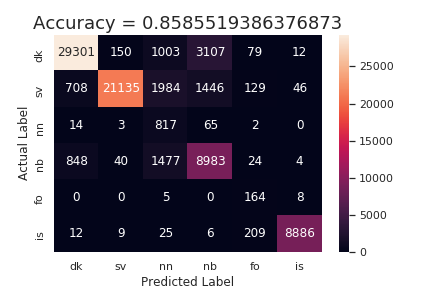
\includegraphics[width=200pt]{figs/fasttextcharngram}
    \caption{Confusion matrix for FastText trained using only characterlevel n-grams on the Wikipedia dataset and evaluated on the tatoeba dataset.}
    \label{fasttextcharngram}
\end{figure}


\subsection{Retraining on the combined dataset}
To improve the accuracy on the Tatoeba dataset I decided to retrain the FastText model on a combined dataset consisting of datapoints from
both the Wikipedia and Tatoeba dataset.\\

The FastText model achieved an accuracy of 97.2\% on this combined dataset and an accuracy of 93.2\% when evaluating this model on the Tatoeba test set alone - the confusion matrix can be seen in Figure \ref{retrain-confuss}.\\

As was the case with the Wikipedia dataset the misclassified sentences tend to be shorter than the average sentence in the dataset. In Figure \ref{retrain-lengths} we see the distribution of sentence lengths for the Tatoeba test set along with the misclassified sentences.\\

 In the Tatoeba test set the mean length of sentences is 37.66 characters with a standard deviation of 17.91 while the mean length is only 29.70 characters for the misclassified sentences with a standard deviation of 9.65. This again supports the conclusion that shorter sentences are harder to classify.

\begin{figure}[h!]
    \begin{subfigure}[b]{0.45\textwidth}
      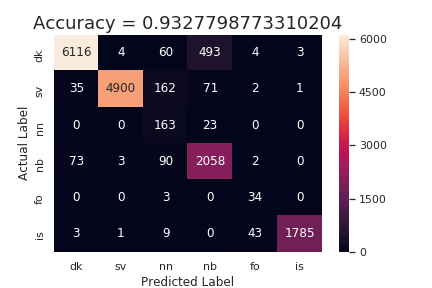
\includegraphics[width=200pt]{figs/retrain}
      \caption{Confusion matrix for FastText trained using only characterlevel n-grams on the combined Wikipedia/Tatoeba dataset and evaluated on the tatoeba dataset.}
      \label{retrain-confuss}
    \end{subfigure}
    ~
    \begin{subfigure}[b]{0.45\textwidth}
        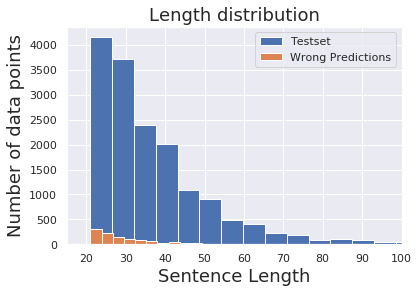
\includegraphics[width=\textwidth]{figs/faliurelengthdist_tatoeba}
        \caption{Distribution of sentence lengths Tatoeba testset along with the misclassified sentences.}
     \label{retrain-lengths}
    \end{subfigure}
\end{figure}


% Not surprisingly we see a substantial increase in performance when including datapoints

% \begin{figure}[h!]
%     \centering
%     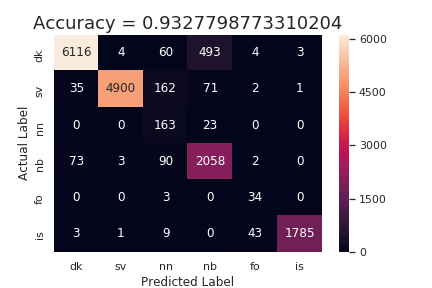
\includegraphics[width=200pt]{figs/retrain}
%     \caption{Confussion matrix for fastText trained using only characterlevel ngrams on the combined Wikipedia/Tatoeba dataset and evaluated on the tatoeba dataset.}
%     \label{retrain}
% \end{figure}



% \begin{figure}
%   \centering
%   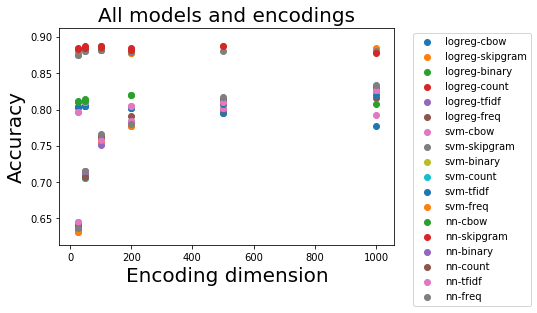
\includegraphics[width = 300pt]{figs/encoding_dimension}
%   \caption{The the performance of the different models.}
%   \label{encodings}
% \end{figure}
%
%
% \begin{figure}
%   \centering
%   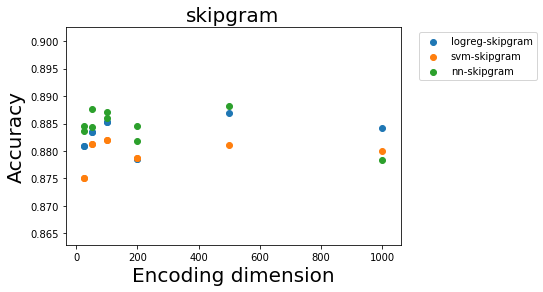
\includegraphics[width = 300pt]{figs/skipgram}
%   \caption{The the performance of the different models.}
%   \label{skipgram}
% \end{figure}
